\documentclass{article}
\usepackage{amsmath}
\usepackage{graphicx}
\begin{document}
\title{Coordinate Geometry Unit Exam: Question 41}
\author{Ana Bhattacharjee}
\date{\today}
\maketitle{}

\begin{center}
We simply plot each coordinate into the equation of a circle.
\begin{align}
  A (-1 , 1) \\
  (-1 + 1)^2 + (1)^2 = 36 \rightarrow 1 < 36
\end{align}
The point is inside the circle.
\begin{align}
  B (-1, 6) \\
  (-1 + 1)^2 + (6)^2 = 36 \rightarrow 36 = 36
\end{align}
The point is on the circle.
\begin{align}
  C (4, -8) \\
  (4 + 1)^2 + (-8)^2 = 36 \rightarrow 25 + 64 > 36
\end{align}
The point is outside on the exterior of the circle.
A visual representation of above is shown below.
\begin{figure}[!htbp]
  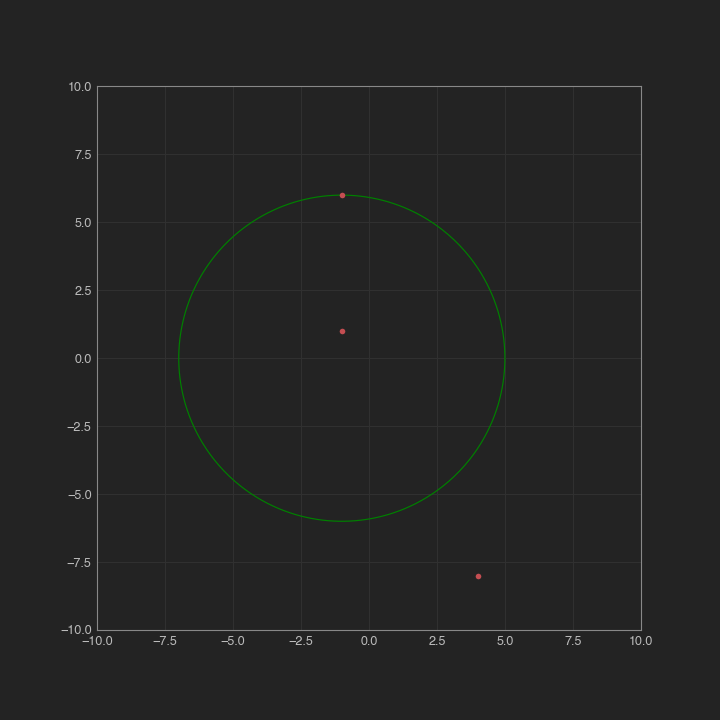
\includegraphics[width=1.0\columnwidth]{circle} 
  \caption{Circle with Points}
\end{figure}
\end{center}
\end{document}
